\subsubsection{1つ前の点を参照する場合}

それぞれの$X_{i}$が、配列の順番が回ってきたときに同じ確率$p$で点を選ぶとしたとき、はじめに与えられた点$x_{0}$のみを参照にしてその点からの近さのみで次の点を選ぶ場合と、一つ前の点のみを参照にして次の点を選ぶ場合の二つの場合に関してシミュレーションを行った。このとき、シミュレーション時に変更できるパラメータとしては、$X_{i}$の数$N$、$X{i}$あたりにもつ点の数$S$、順番が回ってきたときに点を選択する確率$p$がある。

点$x$と$y$の間の近さの指標として、$a$次元ユークリッド距離

\begin{align}D(x, y) &= d(x,y)\\
&= \sqrt{(x_{1} - y_{1})^{2} + (x_{2} - y_{2})^{2} + \cdots + (x_{a} - y_{a})^{2}}\end{align}

を用いることにする。シミュレーションでは、描画の簡単さとイメージのしやすさから$a=2$の場合を考えることにした。

以下に作成したプログラムを用いて得られたネットワークの例を示す(図\ref{fig:f9}, 図\ref{fig:f10})。
図\ref{fig:f9}は、はじめに与えられた点$x_{0}$のみを参照にしたときに得られたネットワークのグラフであり、このとき、中心付近の青色の点は$x_{0}$であり、この点とつながっているエッジは薄い灰色で描画されている。それ以外の黒い線分は、選ばれた意見同士のエッジを表しており、ノードに振られた数字はその点が選ばれた時刻$k$を示している。

\begin{figure}[H]
    \begin{center}
        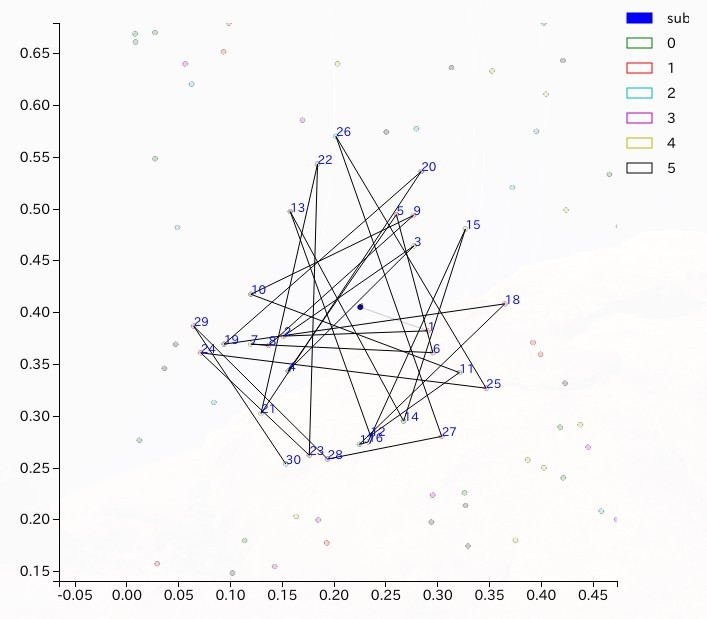
\includegraphics[width=12.5cm]{../simple3/case_2.jpg}
        \caption{$x_{0}$のみを参照にして次の点を選んだ場合のシミュレーション結果の一例}
        \label{fig:f9}
    \end{center}
\end{figure}

\begin{figure}[H]
    \begin{center}
        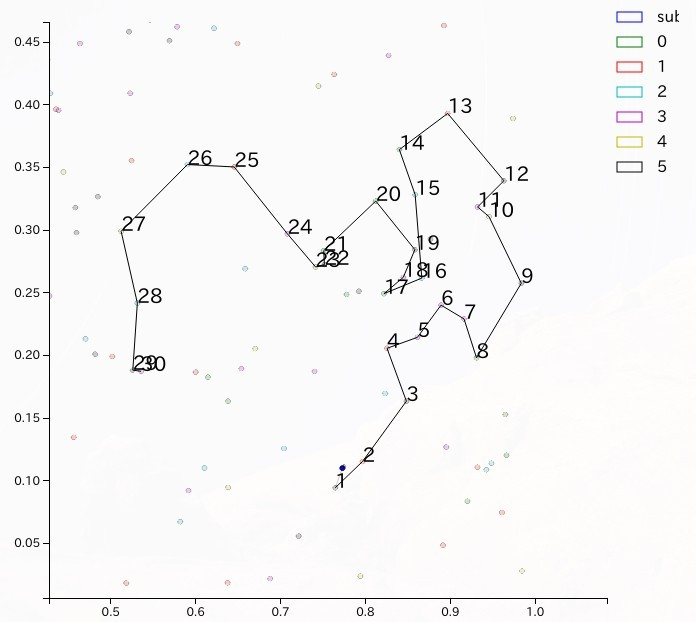
\includegraphics[width=12.5cm]{../simple3/case_3.jpg}
        \caption{1つの点のみを参照にして次の点を選んだ場合のシミュレーション結果の一例}
        \label{fig:f10}
    \end{center}
\end{figure}
